\documentclass[11pt,a4paper]{article}

\usepackage[T1]{fontenc}
\usepackage[utf8]{inputenc}
\usepackage{lmodern}
\usepackage{microtype}
\usepackage[margin=25mm]{geometry}
\usepackage{amsmath,amssymb}
\usepackage{booktabs}
\usepackage{graphicx}
\usepackage{xcolor}
\usepackage{enumitem}
\usepackage[numbers,sort&compress]{natbib}
\usepackage{hyperref}

\hypersetup{
  colorlinks=true,
  linkcolor=black,
  citecolor=blue!50!black,
  urlcolor=blue!50!black,
  pdftitle={Static Loading and Tidal Love Numbers in DSpecM1D},
  pdfauthor={Alex Myhill}
}
\setlist{nosep}
\setlength{\parindent}{0pt}
\setlength{\parskip}{0.55em}
\setcounter{tocdepth}{2}

\newcommand{\code}[1]{\texttt{#1}}
\newcommand{\dd}{\,\mathrm{d}}
\newcommand{\order}{\mathcal{O}}
\newcommand{\relerr}{\varepsilon_{\mathrm{rel}}}

\title{\textbf{Static Loading and Tidal Love Numbers in DSpecM1D}}
\author{Alex Myhill}
\date{\today}

\begin{document}
\hypersetup{pageanchor=false}

\begin{titlepage}
  \centering
  \vspace*{0.20\textheight}
  {\LARGE\bfseries Static Loading and Tidal Love Numbers in
  DSpecM1D\par}
  \vspace{2.0cm}
  {\Large Alex Myhill\par}
  \vspace{0.6cm}
  {\large \today\par}
  \vfill
  \begin{minipage}{0.78\textwidth}
  \small
  This report describes the physical formulation, finite-element
  implementation, user interfaces, and validation evidence for the static
  spheroidal Love-number module.  External programs are treated as independent
  comparisons, not as ground truth.
  \end{minipage}
  \vspace*{0.10\textheight}
\end{titlepage}

\hypersetup{pageanchor=true}
\pagenumbering{roman}
\tableofcontents
\clearpage
\pagenumbering{arabic}

\section{Executive summary}

The DSpecM1D Love-number module computes the static, self-gravitating
spheroidal response of a spherically symmetric, radially transversely
isotropic Earth model.  It supports all-solid structures and arbitrary
internal fluid layers.  The outermost layer must be solid: a surface ocean is
rejected because the required free-surface fluid treatment is outside the
implemented formulation.  Attenuation and rotation are absent.

For each spherical-harmonic degree from zero to a user-selected maximum, the
module solves three independent problems: a unit displacement/traction load,
a unit gravitational-potential load, and a unit tidal potential.  It reports
the dimensional generalized responses
\[
  h_u,\quad k_u,\quad h_\phi,\quad k_\phi,\quad h_t,\quad k_t,
\]
and the physical loading sums
\[
  h_{\mathrm{load}}=h_u+h_\phi,\qquad
  k_{\mathrm{load}}=k_u+k_\phi.
\]
The displacement-type loading quantities \(h_u,h_\phi,h_{\mathrm{load}}\)
have units \(\mathrm{m^3\,kg^{-1}}\); their potential counterparts
\(k_u,k_\phi,k_{\mathrm{load}}\) have units
\(\mathrm{m^4\,kg^{-1}\,s^{-2}}\).  The tidal responses \(h_t\) and \(k_t\)
have units \(\mathrm{s^2\,m^{-1}}\) and one, respectively.

Degree zero is solved as a radial \(U,P\) problem.  A constant degree-zero
tidal potential has zero gradient, so its tidal response is exactly zero.
For degree one the full centre space is retained, but the surface-potential
coefficient is eliminated exactly, imposing \(P(a)=0\).  This fixes the
translation ambiguity in the chosen geocentric frame; it is not the same
post-processing convention used by the ELLN reference software.

Validation proceeds from analytic and algebraic checks to independent
inter-code comparisons.  Constant-density matrices agree with DSpecM1D's
existing radial and spheroidal SEM matrices to roundoff.  Analytic,
piecewise-density tests show that the corrected main-library background
gravity is continuous and accurate to roundoff.  On a controlled internal-fluid
sphere the maximum DSpecM1D--gia3D response difference falls from
\(6.3\times10^{-6}\) at eight elements to \(3.4\times10^{-11}\) at 256
elements.  Sampled isotropized PREM calculations agree at approximately the
\(10^{-7}\) level at the finest common model sampling.  In a degree-10
TI-PREM comparison, using ELLN's gravitational constant explains 68.12\% of
the signed \(h_{10}\) discrepancy and 64.96\% of the signed \(k_{10}\)
discrepancy.  The residual relative difference is about \(1.1\times10^{-4}\);
the exported model agrees with the ELLN definitions to machine precision, so
the remaining difference is recorded as unresolved rather than attributed to
either implementation.

\section{Using the module}

\subsection{CMake configuration}

The module is disabled by default.  Enable it when configuring DSpecM1D:
\begin{verbatim}
cmake -S . -B build -DDSPECM1D_BUILD_LOVE_NUMBERS=ON
cmake --build build --parallel
\end{verbatim}
With tests enabled, the same build registers the normal Love-number test
suite.  The external-reference tests are separately gated by
\code{DSPECM1D\_ENABLE\_PAPER\_VALIDATION}.

\subsection{Command line}

The installed build-tree executable has the positional interface
\begin{verbatim}
dspecm1d-love MODEL_FILE LMAX OUTPUT_FILE \
              [POLYNOMIAL_ORDER] [MAXIMUM_RADIAL_STEP]
\end{verbatim}
The optional polynomial degree defaults to \(p=6\), hence seven
Gauss--Lobatto--Legendre (GLL) nodes per element.  The default maximum
relative radial step is \(0.01\).  An output path of \code{-} writes to
standard output.  Configuration and model errors produce a non-zero exit
status; in particular, a model whose outermost layer is fluid is rejected.

For example, a short no-ocean PREM calculation can be written to standard
output with
\begin{verbatim}
build/bin/dspecm1d-love data/models/prem.200.no.noatten.txt 2 - 4 0.02
\end{verbatim}
The metadata header and first data row have the form
\begin{verbatim}
# DSpecM1D static Love numbers
# maximum_degree: 2
# polynomial_order: 4
# degree_one_convention: P(a) = 0
# columns: l h_u k_u h_phi k_phi h_load k_load h_t k_t
0 -7.2078025353377543e-05 2.5739078430898041e-16 ...
\end{verbatim}
Every data row contains nine whitespace-separated columns:
\[
\begin{array}{c|cccccccc}
l&h_u&k_u&h_\phi&k_\phi&h_{\mathrm{load}}&
k_{\mathrm{load}}&h_t&k_t .
\end{array}
\]
The units are those stated in the executive summary and are repeated in the
file header.  Rows are ordered from \(l=0\) through \code{LMAX}.

\subsection{C++ API}

The public interface is contained in the single header
\code{DSpecM1D/LoveNumbers}.  This minimal program uses the exact public
types and result members:
\begin{verbatim}
#include <DSpecM1D/LoveNumbers>

int main() {
  const EarthModels::ModelInput<double> model(
      "data/models/prem.200.no.noatten.txt");
  const DSpecM1D::LoveNumbers::Config config{
      .maximum_degree = 10,
      .polynomial_order = 6,
      .maximum_radial_step = 0.01,
  };

  const auto results =
      DSpecM1D::LoveNumbers::calculate(model, config);
  for (const auto &result : results) {
    const int degree = result.degree;
    const double h_load = result.h_load();
    const double k_load = result.k_load();
    (void)degree;
    (void)h_load;
    (void)k_load;
  }
}
\end{verbatim}
The returned vector has \code{maximum\_degree + 1} entries in ascending
degree order.  The individual fields are \code{h\_u}, \code{k\_u},
\code{h\_phi}, \code{k\_phi}, \code{h\_t}, and \code{k\_t}; the two loading
sums are member functions.

\section{Mathematical formulation}

\subsection{Assumptions and generalized responses}

The reference state is spherical and in hydrostatic equilibrium.  Solids may
be radially transversely isotropic, described by the five elastic
coefficients \(A,C,F,L,N\).  Internal inviscid fluid regions are permitted,
including a central fluid, but the surface is solid.  The calculation is
static, linear, non-rotating, self-gravitating, and unattenuated.  Only the
scalar spheroidal response is considered; horizontal output and toroidal
response are not part of this module.  These assumptions are consistent with
the variational treatment of self-gravitating loading described by
\citet{alattar_tromp_2014} and its reciprocity extensions
\citep{alattar_et_al_2024}.

For surface radius \(a\), write the radial displacement and Eulerian
potential perturbation of a single harmonic coefficient as
\begin{align}
 u_{lm}(a) &=
 h_{u,l}\,\zeta_{u,lm}
 +h_{\phi,l}\,\zeta_{\phi,lm}
 +h_{t,l}\,\psi_{lm}, \label{eq:general-u}\\
 \phi_{lm}(a) &=
 k_{u,l}\,\zeta_{u,lm}
 +k_{\phi,l}\,\zeta_{\phi,lm}
 +k_{t,l}\,\psi_{lm}. \label{eq:general-p}
\end{align}
Here \(\zeta_u\) denotes the unit displacement/traction forcing,
\(\zeta_\phi\) the unit surface-potential forcing, and \(\psi\) the unit
tidal potential.  The implementation forms these as three columns and solves
them together.  Setting the two generalized loading coefficients equal gives
\begin{equation}
 h_{\mathrm{load},l}=h_{u,l}+h_{\phi,l},\qquad
 k_{\mathrm{load},l}=k_{u,l}+k_{\phi,l}. \label{eq:load-sums}
\end{equation}

\begin{table}[tb]
\centering
\caption{Public response quantities and dimensional units.}
\label{tab:units}
\begin{tabular}{lll}
\toprule
Quantity & Meaning & Unit\\
\midrule
\(h_u,h_\phi,h_{\mathrm{load}}\) & surface radial loading response
  & \(\mathrm{m^3\,kg^{-1}}\)\\
\(k_u,k_\phi,k_{\mathrm{load}}\) & surface potential loading response
  & \(\mathrm{m^4\,kg^{-1}\,s^{-2}}\)\\
\(h_t\) & radial displacement per unit tidal potential
  & \(\mathrm{s^2\,m^{-1}}\)\\
\(k_t\) & potential response per unit tidal potential & 1\\
\bottomrule
\end{tabular}
\end{table}

\subsection{Radial fields and topology}

For \(l\geq1\), each solid region has radial displacement \(U(r)\),
tangential spheroidal displacement \(V(r)\), and potential perturbation
\(P(r)\).  A fluid region has \(P\) only.  Potential is continuous across
every element and material boundary; \(U,V\) are continuous only within each
contiguous solid run.  At a fluid--solid boundary, the solid-side
displacements and the shared potential are independent coefficients.

Degree zero uses continuous radial \(U,P\) fields in both solid and fluid
layers.  At the centre the complete finite-element trial space is retained:
\(U(0),P(0)\) for \(l=0\), and \(U(0),V(0),P(0)\) when the centre is solid
for \(l\geq1\).  No strong-form regularity condition is imposed there.

For degree one, only the surface coefficient \(P(a)\) is removed.  Surface
\(U,V\), every interior potential coefficient, and the complete centre space
remain.  Omitting a basis coefficient is an exact constraint rather than a
penalty; derivatives of all remaining basis functions in the surface element
are still assembled.

\subsection{Solid weak operator}

Let \(q=l(l+1)\), and define the reduced strains
\begin{equation}
 D=rU',\qquad S=rV'-V+U,\qquad T=2U-qV. \label{eq:reduced-strains}
\end{equation}
Hatted symbols denote test fields.  For a solid element and \(l\geq1\), the
implemented symmetric bilinear form is
\begin{align}
\mathcal{K}_{s}=&\int
\bigl[
 C\widehat{D}D
+qL\widehat{S}S
+(A-N)\widehat{T}T
+F(\widehat{D}T+\widehat{T}D)
+q(q-2)N\widehat{V}V \notag\\
&\quad
+4\rho(\pi G\rho r-g)r\,\widehat{U}U
+q\rho gr(\widehat{U}V+\widehat{V}U) \notag\\
&\quad
+\rho r^2(\widehat{U}P'+\widehat{P}'U)
+q\rho r(\widehat{V}P+\widehat{P}V) \notag\\
&\quad
+\frac{r^2\widehat{P}'P'+q\widehat{P}P}{4\pi G}
\bigr]\,\dd r . \label{eq:solid-form}
\end{align}
The first line contains the TI elastic energy; the second contains the
equilibrium-gravity terms; the third couples displacement and potential; and
the last is the gravitational field energy.  The reduced variables in
Eq.~\eqref{eq:reduced-strains} avoid divisions by \(r\) at the centre.
For \(l\geq2\), matching to the exterior vacuum contributes
\begin{equation}
 \mathcal{K}_{\mathrm{vac}}=
 \frac{a(l+1)}{4\pi G}\widehat{P}(a)P(a). \label{eq:vacuum}
\end{equation}
There is no such term for degree one because \(P(a)\) is constrained to zero.

The radial degree-zero form is assembled directly:
\begin{align}
\mathcal{K}_{0}=\int\biggl[
&Cr^2\widehat{U}'U'
+2Fr(\widehat{U}'U+\widehat{U}U') \notag\\
&+4\{\rho(\pi G\rho r-g)r+A-N\}\widehat{U}U \notag\\
&+\rho r^2(\widehat{U}P'+\widehat{P}'U)
+\frac{r^2\widehat{P}'P'}{4\pi G}
\biggr]\dd r
+\frac{a}{4\pi G}\widehat{P}(a)P(a).
\label{eq:radial-form}
\end{align}
This same form applies in solid and fluid elements for \(l=0\); the
potential-only fluid form below is not substituted.

\subsection{Internal fluids and interfaces}

For \(l\geq1\), fluid elements retain the gravitational field-energy term
and add the static stratification contribution
\begin{equation}
\mathcal{K}_{f}=\int\left[
 \frac{r^2\widehat{P}'P'+q\widehat{P}P}{4\pi G}
 +\frac{\rho'}{g}r^2\widehat{P}P
\right]\dd r . \label{eq:fluid-form}
\end{equation}
Here \(\rho'=\dd\rho/\dd r\) is the ordinary one-sided derivative of the
density spline in that fluid layer.  Equation~\eqref{eq:fluid-form} contains
a \emph{positive} coefficient \(+\rho'/g\); because stable density commonly
decreases outwards, its numerical value is often negative.  No additional
minus sign is introduced, and density jumps are not represented as volume
derivatives.  The combined coefficient \(r^2\rho'/g\) is set to zero at
\(r=0\), avoiding \(0/0\).

At a transition radius, let
\[
s=\begin{cases}
-1,&\text{solid below, fluid above},\\
+1,&\text{fluid below, solid above}.
\end{cases}
\]
Using the density \(\rho_f\) on the fluid side and displacement \(U_s\) on
the solid side, the interface term is
\begin{equation}
\mathcal{K}_{\Gamma}=
s\rho_f r^2\left[
g\,\widehat{U}_sU_s+\widehat{U}_sP+\widehat{P}U_s
\right]. \label{eq:interface}
\end{equation}
The orientation is determined explicitly from the adjacent materials, not
from interface parity.  Both directions are tested independently.

\subsection{Forcing and exceptional degrees}

The three load functionals are accumulated first and negated once:
\begin{equation}
 KX=-L. \label{eq:load-sign}
\end{equation}
The displacement and gravitational columns have surface contributions
\begin{equation}
 L_u[\widehat U]=a^2g(a)\widehat U(a),\qquad
 L_\phi[\widehat P]=a^2\widehat P(a). \label{eq:surface-loads}
\end{equation}
The second expression is absent at \(l=1\), where there is no surface
potential test coefficient.  For tide, \(\psi(r)=(r/a)^l\).  Solid elements
contribute
\begin{equation}
 \int \rho r\psi(r)\{l\widehat U+q\widehat V\}\dd r,
\end{equation}
fluid elements contribute
\(\int (r^2\rho'/g)\psi\,\widehat P\,\dd r\), and each interface contributes
\(s\rho_f r^2\psi\,\widehat U_s\).

At \(l=0\), the tidal potential is constant and its gradient vanishes, so the
tidal right-hand side and \(h_t,k_t\) are exactly zero.  At \(l=1\), the
unconstrained static system has a rigid-translation null vector proportional
to \(U=1,V=1,P=-g(r)\).  The exact condition \(P(a)=0\) selects a geocentric
representative without removing centre coefficients.  ELLN instead reports
degree-one values after a deformed-centre transformation.  Its conventional
\(k_1=0\) therefore cannot be obtained by applying the generic
\(l\geq2\) loading conversion to this constrained solution, and degree-one
ELLN comparisons are deliberately excluded.

\section{Numerical implementation}

\subsection{Model, mesh, and finite-element space}

\code{EarthModels::ModelInput<double>} reads a layered radial deck and
constructs splines for density and elastic properties.  DSpecM1D's existing
normalization maps length, density, and time to the nondimensional variables
used in assembly.  \code{RadialState} owns one
\code{EarthMesh::RadialMesh}, the sampled \code{MeshModel}, one-sided
density derivatives, and access to the \code{MeshModel} gravity used
throughout the Love-number calculation.

The mesh is constructed with the existing DSpecM1D relative radial-step
algorithm.  The public \code{polynomial\_order} is the polynomial degree
\(p\), and each element therefore has \(p+1\) GLL nodes.  Material interfaces
are represented by adjacent elements with the same boundary radius but
distinct layer numbers.  Consequently each element samples its own density
spline and its own one-sided derivative at a discontinuity.

\code{LoveDofMap} performs one explicit outward traversal.  Potential
coefficients are shared across all boundaries.  Solid displacement
coefficients are shared across solid--solid boundaries, but are neither
allocated in a fluid nor shared across a fluid gap.  Degree zero interleaves
\(U,P\); a newly encountered solid node for \(l\geq1\) interleaves
\(U,V,P\).  Degree one differs only by omission of surface \(P\).

Element contributions are inserted directly into an Eigen sparse matrix.
For each degree, one \code{SparseLU} factorization solves the three columns
simultaneously.  The same map is used for matrix assembly, forcing, and
surface extraction.  The nondimensional surface values are converted back
using DSpecM1D's \code{LengthNorm}, \code{DensityNorm}, and \code{TimeNorm};
the resulting units are listed in Table~\ref{tab:units}.

\subsection{Corrected background gravity}

The main DSpecM1D \code{MeshModel} background-gravity integration was
corrected in commit
\begin{center}
\code{207b6462ab169a86b7cd4ea183424e2a65d7c34b}.
\end{center}
The authoritative calculation integrates enclosed mass:
\begin{equation}
 I(r)=\int_0^r\rho(s)s^2\dd s,\qquad
 g(r)=\frac{4\pi G I(r)}{r^2},\qquad g(0)=0. \label{eq:gravity}
\end{equation}
Integration is cumulative from the centre, so enclosed mass and gravity are
continuous at every duplicated element and material boundary.  Each interval
is split at the density-spline knots returned for its model layer, and
density is evaluated at the actual quadrature radius.

\code{RadialState::gravity} and \code{surfaceGravity} now delegate directly
to the owned \code{MeshModel}.  The former duplicate private Love-number
integration has been removed, while the operator and forcing continue to use
the same \code{RadialState} accessors.  The current production implementation
therefore has one authoritative gravity calculation.

\section{Validation and benchmarking}

\subsection{Evidence hierarchy and reproducibility}

The validation hierarchy is:
\begin{enumerate}
\item focused topology, sign, symmetry, forcing, solve, units, and API tests;
\item analytic gravity tests for homogeneous and piecewise-density spheres;
\item constant-density matrix oracles using DSpecM1D
      \code{hR()} and \code{hS(l)};
\item matched homogeneous and controlled-fluid comparisons with gia3D;
\item a three-way isotropized-PREM comparison with gia3D; and
\item a TI-PREM loading comparison with the official ELLN software.
\end{enumerate}
The final two levels are independent comparisons rather than exact
regression oracles.  The gia3D solid matrix is isotropic, so it cannot
validate the complete TI operator.  Conversely, ELLN reports conventional
loading \(h_l,l_l,k_l\), not the separate generalized and tidal responses.
The horizontal \(l_l\) is not exposed by the DSpecM1D public API.
The software revisions and publisher package are cited separately from their
associated mathematical papers
\citep{gia3d_software,gia3d_core_software,elln_supporting_information}.

The CSV files behind every figure begin with model, resolution, quantity, and
source-script metadata.  They are regenerated from labelled validation
outputs by \code{collect\_benchmarks.py}; the plotting script contains no
Love-number or gravity calculation.  Exact commands are listed in
\code{report/README.md}.

\subsection{Analytic gravity and controlled models}

Figure~\ref{fig:gravity} compares current background gravity on the
controlled solid--fluid--solid sphere with its piecewise analytic value.
The DSpecM1D error remains between \(1.8\times10^{-15}\) and
\(1.1\times10^{-14}\,\mathrm{m\,s^{-2}}\), while gia3D converges towards its
roundoff/discretisation floor.  An earlier \code{MeshModel} quadrature defect
was identified during Love-number validation and corrected in commit
\code{207b6462ab169a86b7cd4ea183424e2a65d7c34b}.  Current Love-number
calculations use that corrected shared implementation; the obsolete
defective-output curve is no longer retained as an active benchmark.

\begin{figure}[!htbp]
\centering
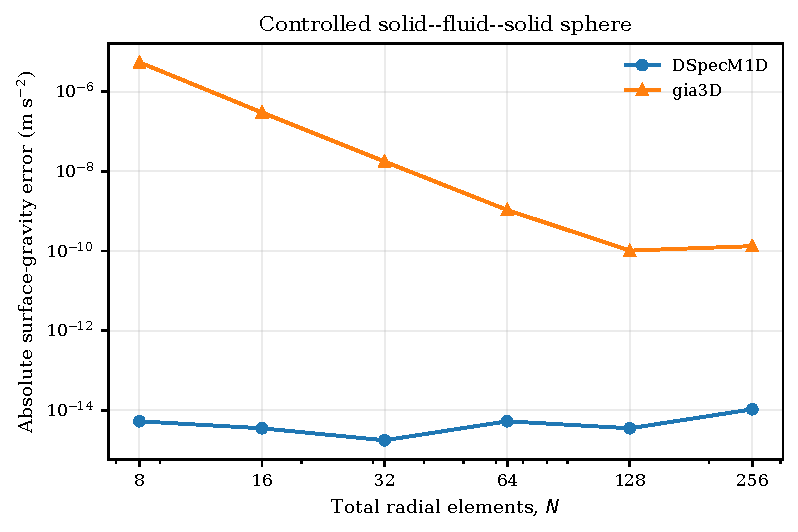
\includegraphics[width=0.86\textwidth]{figures/background_gravity_current.pdf}
\caption{Absolute surface-gravity error for the controlled
solid--fluid--solid density profile.  DSpecM1D uses the corrected shared
\code{MeshModel} implementation; gia3D is the pinned independent reference.
Both errors are measured against the piecewise analytic density integral.}
\label{fig:gravity}
\end{figure}

With the corrected gravity, the response comparison converges steadily
(Figure~\ref{fig:controlled-fluid}).  At \(N=256\), the maximum
component-wise relative differences are \(1.45\times10^{-11}\),
\(3.37\times10^{-11}\), and \(1.58\times10^{-11}\) for degrees 1, 2, and
10.  This is close to the solve-residual scale at that large system size and
approaches the homogeneous-sphere solver agreement.

\begin{figure}[p]
\centering
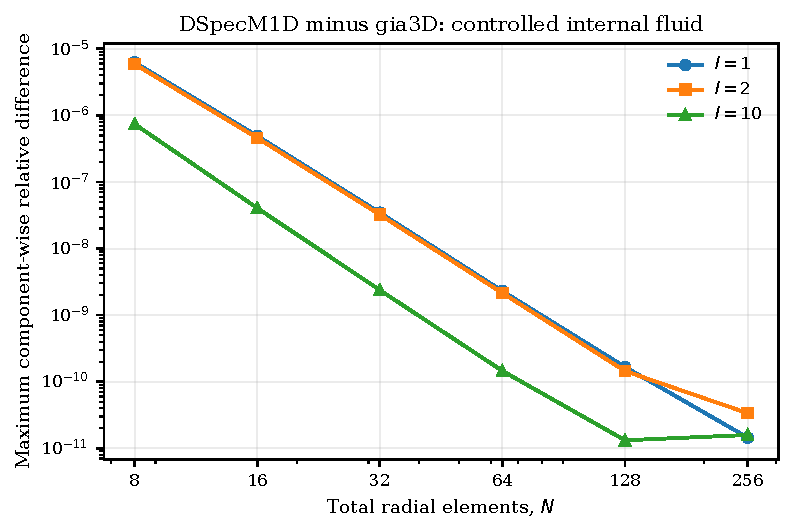
\includegraphics[width=0.86\textwidth]{figures/controlled_fluid_convergence.pdf}
\caption{Maximum relative difference over the eight reported response
components for matched solid--fluid--solid meshes in DSpecM1D and gia3D.
Both interface orientations and a non-zero negative fluid density derivative
are present.}
\label{fig:controlled-fluid}
\end{figure}

\begin{table}[tb]
\centering
\caption{Finest controlled-model inter-code diagnostics.  The reported
difference is the maximum over all eight response components; residuals are
the maximum over the three simultaneous solves.}
\label{tab:controlled}
\small
\begin{tabular}{llrrrr}
\toprule
Model & \(l\) & \(N\) & max.\ rel.\ diff. &
DSpecM1D residual & \(|\)DSpec reciprocity\(|\)\\
\midrule
Homogeneous & 1  & 32  & \(7.14\,10^{-13}\) & \(7.38\,10^{-13}\) & 0\\
            & 2  & 32  & \(4.01\,10^{-12}\) & \(3.99\,10^{-12}\) & \(2.83\,10^{-12}\)\\
            & 10 & 32  & \(5.72\,10^{-13}\) & \(1.89\,10^{-13}\) & \(9.99\,10^{-15}\)\\
Central fluid & 1  & 32 & \(5.32\,10^{-8}\) & \(6.11\,10^{-13}\) & 0\\
              & 2  & 32 & \(5.06\,10^{-8}\) & \(6.03\,10^{-12}\) & \(1.73\,10^{-12}\)\\
              & 10 & 32 & \(3.22\,10^{-9}\) & \(1.85\,10^{-13}\) & \(7.04\,10^{-13}\)\\
Solid--fluid--solid & 1 & 256 & \(1.45\,10^{-11}\) & \(1.50\,10^{-11}\) & 0\\
                    & 2 & 256 & \(3.37\,10^{-11}\) & \(1.32\,10^{-10}\) & \(7.79\,10^{-13}\)\\
                    & 10& 256 & \(1.58\,10^{-11}\) & \(3.62\,10^{-12}\) & \(3.44\,10^{-15}\)\\
\bottomrule
\end{tabular}
\end{table}

The central-fluid results and all assembled entries remain finite at
\(r=0\).  Their \(N=32\) inter-code differences are larger than the
homogeneous results but still decrease with refinement; no invalid
floating-point condition or unintended empty matrix row is observed.
Reciprocity is assessed from \(g(a)h_\phi-k_u\) in dimensional SI units and
is zero for the constrained degree-one columns.

\subsection{Isotropized PREM}

The isotropized-PREM experiment separates three effects.  gia3D first
evaluates its analytic PREM representation.  The same exporter creates
paired isotropic decks, which are then read independently by gia3D and
DSpecM1D.  Figure~\ref{fig:isotropic-prem} shows the maximum response
difference over degrees \(1,2,10,50\) at common radial step \(0.0025\).
The sampled-code difference falls from \(2.27\times10^{-5}\) at 100-km
knots to \(1.55\times10^{-7}\) at 12.5-km knots.  The sampled gia3D--analytic
PREM difference follows almost the same trend, demonstrating that model
interpolation, rather than either linear solve alone, controls the plateau.

\begin{figure}[!htbp]
\centering
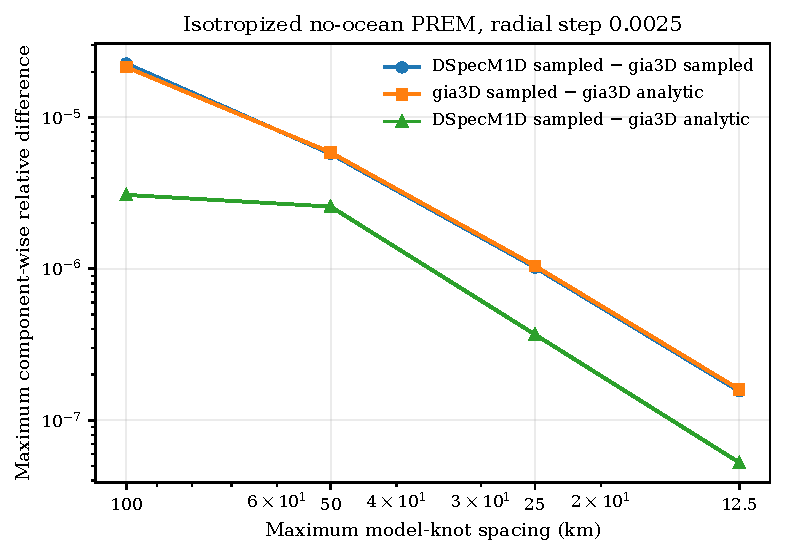
\includegraphics[width=0.86\textwidth]{figures/isotropic_prem_convergence.pdf}
\caption{Maximum component-wise relative differences for the three-way
isotropized no-ocean PREM comparison at radial step 0.0025.  Both sampled
calculations approximate, rather than reproduce exactly, gia3D's analytic
PREM representation.}
\label{fig:isotropic-prem}
\end{figure}

\begin{table}[tb]
\centering
\caption{Largest component-wise relative difference in each direction for
the finest 12.5-km isotropized-PREM deck at radial step 0.0025.}
\label{tab:isotropic-prem}
\small
\begin{tabular}{lrrr}
\toprule
Difference & \(l\) & component & relative difference\\
\midrule
DSpec sampled \(-\) gia3D sampled & 10 & \(k_u\) & \(+1.5540\,10^{-7}\)\\
gia3D sampled \(-\) gia3D analytic & 10 & \(k_u\) & \(-1.5963\,10^{-7}\)\\
DSpec sampled \(-\) gia3D analytic & 50 & \(k_t\) & \(-5.2471\,10^{-8}\)\\
\bottomrule
\end{tabular}
\end{table}

At this resolution the sampled DSpecM1D systems have 3728 degrees of freedom
for \(l=1\) and 3729 otherwise; gia3D's sampled and analytic systems have
3616 and 3617.  The difference follows their distinct layer meshing while
the reported surface radius is common.  Maximum three-column residuals are
\(3.6\times10^{-11}\), \(2.2\times10^{-10}\),
\(5.1\times10^{-12}\), and \(1.1\times10^{-12}\) for DSpecM1D degrees
1, 2, 10, and 50.  The largest absolute DSpecM1D reciprocity diagnostic is
\(3.36\times10^{-13}\).  These algebraic errors are below the model-sampling
differences.

\subsection{TI-PREM and the gravitational constant}

The official Chen--Pan--Bevis ELLN calculation
\citep{chen_pan_bevis_2018} supplies an independent TI loading comparison.
The ELLN mantle coefficients map directly as
\[
 A=c_{11},\quad C=c_{33},\quad F=c_{13},\quad
 L=c_{44},\quad N=c_{66}.
\]
Its analytic layer definitions were sampled into a DSpecM1D deck down to
6.25-km knot spacing.  Selected audits on both sides of boundaries found a
maximum elastic-coefficient relative mismatch of \(6.61\times10^{-16}\).
ELLN uses \(G=6.67384\times10^{-11}\) SI, while production DSpecM1D uses
\(6.67230\times10^{-11}\) SI, a relative difference of
\(2.30805\times10^{-4}\).

\begin{table}[tb]
\centering
\caption{Degree-10 comparison with ELLN Table S7 at \(p=6\), maximum radial
step 0.00125, and 6.25-km model knots.  Signed differences are
DSpecM1D minus the published value.}
\label{tab:elln}
\begin{tabular}{lrrrr}
\toprule
Case & \(h_{10}\) & \(\Delta h_{10}/|h_{10}^{S7}|\) &
\(k_{10}\) & \(\Delta k_{10}/|k_{10}^{S7}|\)\\
\midrule
Table S7 & \(-1.451586\) & --- & \(-0.07066685\) & ---\\
Production \(G\) & \(-1.45109447\) & \(3.3862\,10^{-4}\) &
  \(-0.0706430844\) & \(3.3630\,10^{-4}\)\\
ELLN \(G\) & \(-1.45142929\) & \(1.0796\,10^{-4}\) &
  \(-0.0706585226\) & \(1.1784\,10^{-4}\)\\
\bottomrule
\end{tabular}
\end{table}

\begin{figure}[!htbp]
\centering
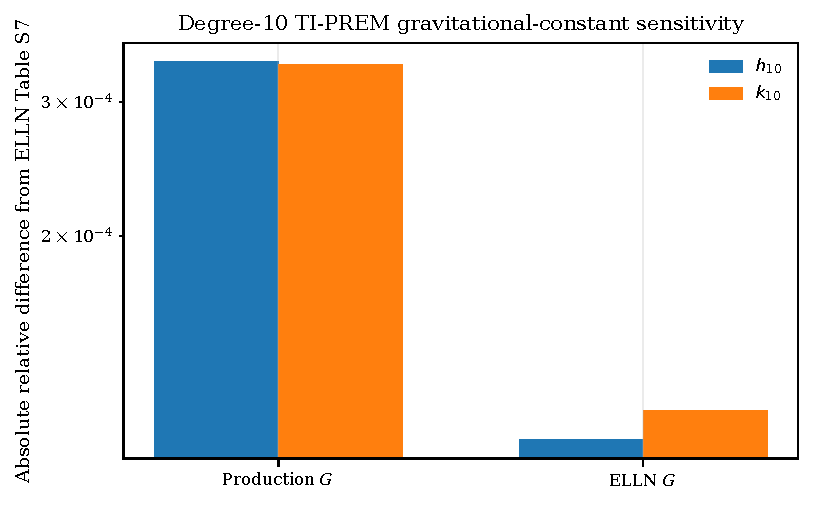
\includegraphics[width=0.68\textwidth]{figures/elln_gravitational_constant.pdf}
\caption{Absolute relative degree-10 discrepancy from ELLN Table S7 using
the production gravitational constant and a validation-only source copy
patched consistently to ELLN's constant.  The comparison changes only
physical \(G\), not the source-tree implementation or model normalization.}
\label{fig:elln-g}
\end{figure}

Matching \(G\) explains 68.12\% of the signed \(h_{10}\) discrepancy and
64.96\% of the signed \(k_{10}\) discrepancy
(Figure~\ref{fig:elln-g}).  The production and matched-\(G\) maximum solve
residuals are \(3.44\times10^{-11}\) and \(3.47\times10^{-11}\);
absolute reciprocity errors are \(3.78\times10^{-14}\) and
\(4.43\times10^{-14}\).  Thus the remaining \(1.1\times10^{-4}\)-scale
difference is much larger than the algebraic solve errors but is not explained
by a detected model transcription error.  Possible representation,
tabulation, or inter-code differences remain unresolved.  Agreement or
disagreement with ELLN alone is not evidence that either calculation is
correct or incorrect.

\subsection{External provenance and limitations}

\begin{table}[tb]
\centering
\caption{Pinned external validation inputs.  The ELLN archive is not
vendored because no redistribution licence was found.}
\label{tab:provenance}
\small
\begin{tabular}{lll}
\toprule
Input & Revision or SHA-256 & Role\\
\midrule
\code{da380/gia3D} &
\code{e6a8230fc792416087e530726e3f9f9b41ee0506} &
isotropic reference\\
\code{da380/core} &
\code{eb1d36e418ab0ac9e0b34abb717e6d9b2e863ee5} &
gia3D support\\
\code{ggx444\_supp.zip} &
\code{f2904364f9be96239fc85140a032b01b7}\ldots &
official ELLN package\\
\bottomrule
\end{tabular}
\end{table}

The paper-validation build copies and patches pinned sources in its build
tree only.  Two small gia3D patches initialize the fluid quadrature radius
before evaluating \(r^2\rho'/g\) and make the central tidal coefficient safe
at \(r=0\).  A separate ELLN compatibility patch suppresses GUI waitbars for
non-interactive reproduction.  The gravitational-constant experiment copies
the Love-number source to the build tree and changes the one physical
constant consistently in gravity, operator, forcing, and conventional
conversion paths.  None of these changes modifies production source.

The published \code{love.dat} subset is retained as a diagnostic, not an
exact oracle: gia3D uses analytic PREM coefficients and an isotropic solid
matrix, whereas the earlier local deck is sampled and can be TI.  ELLN's
degree-one frame is not equivalent to \(P(a)=0\), and its horizontal response
cannot presently be compared.  No external comparison covers a surface
ocean, which remains unsupported.  Broader formulations, including
full-domain gravitation techniques such as those discussed by
\citet{yu_et_al_2026}, are outside this static radial module.

\clearpage
\appendix
\section*{Appendix A: Love-number test inventory}
\addcontentsline{toc}{section}{Appendix A: Love-number test inventory}
\label{app:tests}

The following 66 entries are generated from \code{love\_numbers/TESTS.md}.
They correspond exactly to the Love-number registrations in a fresh
paper-validation CTest listing: 55 normal tests and 11 gated
paper-validation tests.  Unrelated core DSpecM1D tests are omitted.

\setlength{\emergencystretch}{2em}
\sloppy
% Generated from ../TESTS.md by generate_test_appendix.py.
\small
\subsection*{Radial state, material model, and gravity}
\begin{itemize}[leftmargin=1.4em,itemsep=0.35em]
\item {\footnotesize\texttt{RadialStateTests.PolynomialOrderUsesOneMoreGllNode}}\\
\emph{normal; \texttt{tests/test\_radial\_state.cpp}.} Checks that polynomial degree \texttt{p} creates exactly \texttt{p+1} GLL nodes per element.
\item {\footnotesize\texttt{RadialStateTests.MeshEndsAtSurfaceWithoutExteriorBall}}\\
\emph{normal; \texttt{tests/test\_radial\_state.cpp}.} Checks that the mesh contains no exterior ball and ends at the model outer radius.
\item {\footnotesize\texttt{RadialStateTests.SampledModelValuesAreFinite}}\\
\emph{normal; \texttt{tests/test\_radial\_state.cpp}.} Samples density, TI moduli, gravity, and the density derivative at every element node and requires finite values.
\item {\footnotesize\texttt{RadialStateTests.HomogeneousSphereGravityIsAnalyticAtEveryNode}}\\
\emph{normal; \texttt{tests/test\_radial\_state.cpp}.} Compares every nodal gravity value with the homogeneous-sphere analytic solution, including the finite zero at the centre.
\item {\footnotesize\texttt{RadialStateTests.ControlledSolidFluidSolidGravityIsAnalytic}}\\
\emph{normal; \texttt{tests/test\_radial\_state.cpp}.} Compares nodal gravity with the piecewise analytic solid--fluid--solid density integral.
\item {\footnotesize\texttt{RadialStateTests.MinimumPolynomialOrderExactlyIntegratesCubicDensityGravity}}\\
\emph{normal; \texttt{tests/test\_radial\_state.cpp}.} Checks roundoff-level analytic surface gravity for cubic density at the minimum polynomial order \texttt{p=3}.
\item {\footnotesize\texttt{RadialStateTests.ControlledCentralFluidGravityIsAnalytic}}\\
\emph{normal; \texttt{tests/test\_radial\_state.cpp}.} Checks the analytic gravity of a constant-density central fluid and solid exterior.
\item {\footnotesize\texttt{RadialStateTests.GravityIsContinuousAcrossEveryBoundary}}\\
\emph{normal; \texttt{tests/test\_radial\_state.cpp}.} Requires identical gravity values on both copies of every element and material boundary.
\item {\footnotesize\texttt{RadialStateTests.DensityDerivativeUsesElementLayerSpline}}\\
\emph{normal; \texttt{tests/test\_radial\_state.cpp}.} Compares each sampled derivative with the derivative of that element's density spline.
\item {\footnotesize\texttt{RadialStateTests.MaterialInterfaceUsesOneSidedDensityDerivatives}}\\
\emph{normal; \texttt{tests/test\_radial\_state.cpp}.} Checks that duplicated-radius interface nodes use the lower and upper layer derivatives independently.
\item {\footnotesize\texttt{RadialStateTests.RejectsSurfaceFluid}}\\
\emph{normal; \texttt{tests/test\_radial\_state.cpp}.} Requires a clear exception when the outermost layer is fluid.
\item {\footnotesize\texttt{RadialStateTests.RejectsInvalidConfiguration}}\\
\emph{normal; \texttt{tests/test\_radial\_state.cpp}.} Rejects negative maximum degree and non-positive radial step.
\end{itemize}
\subsection*{DOF mapping}
\begin{itemize}[leftmargin=1.4em,itemsep=0.35em]
\item {\footnotesize\texttt{LoveDofMapTests.DegreeZeroInterleavesEveryNodeAndMatchesRadialSemMap}}\\
\emph{normal; \texttt{tests/test\_love\_dof\_map.cpp}.} Checks continuous interleaved \texttt{U,P} indexing and exact agreement with the existing radial SEM map.
\item {\footnotesize\texttt{LoveDofMapTests.DegreeZeroRetainsCentreFields}}\\
\emph{normal; \texttt{tests/test\_love\_dof\_map.cpp}.} Verifies independent \texttt{U(0)} and \texttt{P(0)} coefficients.
\item {\footnotesize\texttt{LoveDofMapTests.AllSolidDegreeTwoInterleavesEveryField}}\\
\emph{normal; \texttt{tests/test\_love\_dof\_map.cpp}.} Checks all-solid \texttt{U,V,P} interleaving, dimension, and exact agreement with the existing spheroidal SEM map.
\item {\footnotesize\texttt{LoveDofMapTests.SolidCentreRetainsThreeIndependentFields}}\\
\emph{normal; \texttt{tests/test\_love\_dof\_map.cpp}.} Verifies independent \texttt{U(0)}, \texttt{V(0)}, and \texttt{P(0)} coefficients.
\item {\footnotesize\texttt{LoveDofMapTests.PotentialIsSharedAcrossEveryElementBoundary}}\\
\emph{normal; \texttt{tests/test\_love\_dof\_map.cpp}.} Checks continuity of the single potential coefficient across solid, fluid, and material boundaries.
\item {\footnotesize\texttt{LoveDofMapTests.DisplacementsAreSharedAcrossSolidBoundaries}}\\
\emph{normal; \texttt{tests/test\_love\_dof\_map.cpp}.} Checks that adjacent solid elements share their \texttt{U} and \texttt{V} boundary coefficients.
\item {\footnotesize\texttt{LoveDofMapTests.DisplacementsAreAbsentFromFluidElements}}\\
\emph{normal; \texttt{tests/test\_love\_dof\_map.cpp}.} Requires \texttt{U} and \texttt{V} to return \texttt{nullopt} at every fluid node.
\item {\footnotesize\texttt{LoveDofMapTests.InterfacesKeepDisplacementsOnlyOnSolidSide}}\\
\emph{normal; \texttt{tests/test\_love\_dof\_map.cpp}.} Exercises both interface orientations and checks that displacement exists only on the solid side while \texttt{P} is shared.
\item {\footnotesize\texttt{LoveDofMapTests.InternalFluidDimensionsMatchTopologyFormulas}}\\
\emph{normal; \texttt{tests/test\_love\_dof\_map.cpp}.} Compares explicit map sizes with the radial-node and separate-solid-run dimension formulas.
\item {\footnotesize\texttt{LoveDofMapTests.DegreeOneOnlyOmitsSurfacePotential}}\\
\emph{normal; \texttt{tests/test\_love\_dof\_map.cpp}.} Compares degree one and degree two and requires the sole missing coefficient to be surface \texttt{P}.
\item {\footnotesize\texttt{LoveDofMapTests.DegreeOneRetainsSurfaceDisplacements}}\\
\emph{normal; \texttt{tests/test\_love\_dof\_map.cpp}.} Verifies that degree-one surface \texttt{U} and \texttt{V} remain present.
\item {\footnotesize\texttt{LoveDofMapTests.RejectsNegativeDegree}}\\
\emph{normal; \texttt{tests/test\_love\_dof\_map.cpp}.} Requires a negative degree to throw \texttt{std::invalid\_argument}.
\end{itemize}
\subsection*{All-solid operator}
\begin{itemize}[leftmargin=1.4em,itemsep=0.35em]
\item {\footnotesize\texttt{StaticOperatorTests.MatchesIsotropicReference}}\\
\emph{normal; \texttt{tests/test\_static\_operator.cpp}.} Compares degree 2 and 10 isotropic matrices with \texttt{Full1D::SEM::hS(l)}, including dimensions and roundoff symmetry.
\item {\footnotesize\texttt{StaticOperatorTests.MatchesTransverselyIsotropicReference}}\\
\emph{normal; \texttt{tests/test\_static\_operator.cpp}.} Repeats the degree 2 and 10 \texttt{hS(l)} matrix comparison for a genuinely TI constant-density model.
\item {\footnotesize\texttt{StaticOperatorTests.RetainsCentreFieldsAndMatchesSemOrdering}}\\
\emph{normal; \texttt{tests/test\_static\_operator.cpp}.} Checks the three centre coefficients and exact all-solid SEM ordering.
\item {\footnotesize\texttt{StaticOperatorTests.RejectsNegativeDegree}}\\
\emph{normal; \texttt{tests/test\_static\_operator.cpp}.} Requires the private static operator to reject a negative degree.
\end{itemize}
\subsection*{Fluid operator and interfaces}
\begin{itemize}[leftmargin=1.4em,itemsep=0.35em]
\item {\footnotesize\texttt{StaticFluidOperatorTests.InterfaceSignsUseFluidSideDensity}}\\
\emph{normal; \texttt{tests/test\_static\_fluids.cpp}.} Isolates both solid--fluid interface orientations and verifies sign, fluid-side density, shared \texttt{P}, and solid-side \texttt{U}.
\item {\footnotesize\texttt{StaticFluidOperatorTests.NonconstantFluidBlockUsesPositiveDensityGradient}}\\
\emph{normal; \texttt{tests/test\_static\_fluids.cpp}.} Compares the fluid potential block with an independent quadrature assembly containing \texttt{+r\textasciicircum{}2 rho'/g}.
\item {\footnotesize\texttt{StaticFluidOperatorTests.ConstantDensityCentralFluidIsFinite}}\\
\emph{normal; \texttt{tests/test\_static\_fluids.cpp}.} Checks zero stratification, a finite central-fluid matrix, and safe handling of \texttt{r=g=0}.
\item {\footnotesize\texttt{StaticFluidOperatorTests.InternalFluidMatricesAreCompleteAndSymmetric}}\\
\emph{normal; \texttt{tests/test\_static\_fluids.cpp}.} Requires internal-fluid and no-ocean PREM matrices to have the map dimension, roundoff symmetry, and no empty row or column.
\end{itemize}
\subsection*{Forcing, solve, residuals, and reciprocity}
\begin{itemize}[leftmargin=1.4em,itemsep=0.35em]
\item {\footnotesize\texttt{StaticForcingTests.SurfaceLoadsHaveExpectedEntriesAndSigns}}\\
\emph{normal; \texttt{tests/test\_static\_solve.cpp}.} Checks the displacement and gravitational surface load entries after the single \texttt{KX=-L} negation.
\item {\footnotesize\texttt{StaticForcingTests.AllSolidTideMatchesIndependentAssembly}}\\
\emph{normal; \texttt{tests/test\_static\_solve.cpp}.} Compares the all-solid tidal column with a test-local GLL assembly at degrees 2 and 10.
\item {\footnotesize\texttt{StaticForcingTests.InternalFluidTideMatchesBothInterfaceOrientations}}\\
\emph{normal; \texttt{tests/test\_static\_solve.cpp}.} Independently assembles solid, fluid-gradient, and both oriented interface tidal terms.
\item {\footnotesize\texttt{StaticSolveTests.OneFactorizationSolvesAllColumnsAndExtractsResults}}\\
\emph{normal; \texttt{tests/test\_static\_solve.cpp}.} Checks three-column residuals, combined-load linearity, dimensional extraction, reciprocity, and finite results for isotropic, TI, fluid, and PREM models.
\item {\footnotesize\texttt{StaticSolveTests.RejectsNegativeDegree}}\\
\emph{normal; \texttt{tests/test\_static\_solve.cpp}.} Requires the private solve function to reject a negative degree.
\end{itemize}
\subsection*{Degree zero}
\begin{itemize}[leftmargin=1.4em,itemsep=0.35em]
\item {\footnotesize\texttt{StaticRadialOperatorTests.MatchesRadialSemForSupportedModels}}\\
\emph{normal; \texttt{tests/test\_static\_radial.cpp}.} Compares degree-zero matrices with \texttt{Full1D::SEM::hR()} for constant-density isotropic and TI models, with symmetry and ordering checks.
\item {\footnotesize\texttt{StaticRadialOperatorTests.RetainsCentreFields}}\\
\emph{normal; \texttt{tests/test\_static\_radial.cpp}.} Verifies independent radial \texttt{U(0)} and \texttt{P(0)} coefficients.
\item {\footnotesize\texttt{StaticRadialForcingTests.SurfaceLoadsAndZeroTideAreExact}}\\
\emph{normal; \texttt{tests/test\_static\_radial.cpp}.} Checks the two surface loads and requires an identically zero degree-zero tidal column.
\item {\footnotesize\texttt{StaticRadialSolveTests.SolvesSupportedModels}}\\
\emph{normal; \texttt{tests/test\_static\_radial.cpp}.} Checks degree-zero residuals, reciprocity, finite model coverage, and exact zero \texttt{h\_t,k\_t}.
\end{itemize}
\subsection*{Degree one}
\begin{itemize}[leftmargin=1.4em,itemsep=0.35em]
\item {\footnotesize\texttt{StaticDegreeOneOperatorTests.AllSolidMatricesMatchConstrainedSem}}\\
\emph{normal; \texttt{tests/test\_static\_degree\_one.cpp}.} Compares isotropic and TI matrices with the principal submatrix of \texttt{hS(1)} after removing surface \texttt{P}, and evaluates the full translation null vector.
\item {\footnotesize\texttt{StaticDegreeOneOperatorTests.RetainsCentreAndSurfaceFields}}\\
\emph{normal; \texttt{tests/test\_static\_degree\_one.cpp}.} Checks independent centre \texttt{U,V,P}, retained surface \texttt{U,V}, and absent surface \texttt{P}.
\item {\footnotesize\texttt{StaticDegreeOneOperatorTests.InternalFluidMatricesHaveExpectedSizeAndSymmetry}}\\
\emph{normal; \texttt{tests/test\_static\_degree\_one.cpp}.} Checks map dimension and roundoff symmetry for an internal fluid and no-ocean PREM.
\item {\footnotesize\texttt{StaticDegreeOneForcingTests.SurfaceLoadsAndIndependentTidesAreCorrect}}\\
\emph{normal; \texttt{tests/test\_static\_degree\_one.cpp}.} Verifies the displacement load, exactly zero gravitational column, and independent all-solid and fluid tidal assemblies.
\item {\footnotesize\texttt{StaticDegreeOneSolveTests.SolvesSupportedModels}}\\
\emph{normal; \texttt{tests/test\_static\_degree\_one.cpp}.} Checks constrained residuals, finite remaining responses, and exact zero potential-related outputs.
\end{itemize}
\subsection*{Public API}
\begin{itemize}[leftmargin=1.4em,itemsep=0.35em]
\item {\footnotesize\texttt{LoveNumbersTests.LoadSumsCombineGeneralizedResponses}}\\
\emph{normal; \texttt{tests/test\_love\_numbers.cpp}.} Checks that \texttt{h\_load()} and \texttt{k\_load()} return the sums of their generalized components.
\item {\footnotesize\texttt{LoveNumbersTests.PublicHeaderCalculatesOrderedDegreeRange}}\\
\emph{normal; \texttt{tests/test\_love\_numbers.cpp}.} Uses only the public header and checks an ordered result for every degree from zero through the configured maximum.
\item {\footnotesize\texttt{LoveNumbersTests.MaximumDegreeZeroIsValid}}\\
\emph{normal; \texttt{tests/test\_love\_numbers.cpp}.} Checks that a degree-zero-only public calculation succeeds and returns one result.
\item {\footnotesize\texttt{LoveNumbersTests.SupportedModelsReturnFiniteValues}}\\
\emph{normal; \texttt{tests/test\_love\_numbers.cpp}.} Runs the public API on isotropic, TI, internal-fluid, and no-ocean PREM models and checks special-degree zeros and finite values.
\item {\footnotesize\texttt{LoveNumbersTests.RejectsInvalidConfigurationAndSurfaceFluid}}\\
\emph{normal; \texttt{tests/test\_love\_numbers.cpp}.} Checks public rejection of invalid configuration values and a surface fluid.
\item {\footnotesize\texttt{LoveNumbersTests.EnforcesMinimumPolynomialOrder}}\\
\emph{normal; \texttt{tests/test\_love\_numbers.cpp}.} Requires the public calculation to reject polynomial orders below three and accept \texttt{p=3}.
\item {\footnotesize\texttt{LoveNumbersPublicPrivateTests.PublicResultsMatchPrivateSolves}}\\
\emph{normal; \texttt{tests/test\_public\_private.cpp}.} Compares every public component directly with private solves at selected degrees including 0, 1, 2, and 10.
\end{itemize}
\subsection*{CLI}
\begin{itemize}[leftmargin=1.4em,itemsep=0.35em]
\item {\footnotesize\texttt{LoveNumbersCliTests.ExplicitOptionsWriteFileAndMatchPublicResults}}\\
\emph{normal; \texttt{tests/test\_cli.cpp}.} Runs explicit optional arguments, parses the file metadata and nine columns, and compares every value with \texttt{calculate}.
\item {\footnotesize\texttt{LoveNumbersCliTests.DefaultsWriteStandardOutput}}\\
\emph{normal; \texttt{tests/test\_cli.cpp}.} Runs the default polynomial order and radial step through standard output and checks ordered rows.
\item {\footnotesize\texttt{LoveNumbersCliTests.InvalidArgumentsAndMissingModelFail}}\\
\emph{normal; \texttt{tests/test\_cli.cpp}.} Requires non-zero status and clear diagnostics for malformed arguments and a missing model.
\item {\footnotesize\texttt{LoveNumbersCliTests.RejectsUnderintegratedPolynomialOrders}}\\
\emph{normal; \texttt{tests/test\_cli.cpp}.} Requires non-zero status and the \texttt{p >= 3} diagnostic for \texttt{p=1} and \texttt{p=2}.
\item {\footnotesize\texttt{LoveNumbersCliTests.SurfaceFluidIsRejectedClearly}}\\
\emph{normal; \texttt{tests/test\_cli.cpp}.} Runs the CLI on a surface-fluid model and checks the explicit no-ocean error.
\end{itemize}
\subsection*{gia3D validation}
\begin{itemize}[leftmargin=1.4em,itemsep=0.35em]
\item {\footnotesize\texttt{LoveNumbersGia3DReference.ReportsDirectComparison}}\\
\emph{paper validation; \texttt{validation/gia3d/compare\_reference.py}.} Runs the pinned original-truncation PREM driver, reports three independent solutions and stock combined-load agreement, and requires finite residuals and degree-one zeros.
\item {\footnotesize\texttt{LoveNumbersGia3DReference.ReportsControlledSphereComparison}}\\
\emph{paper validation; \texttt{validation/compare\_controlled\_sphere.py}.} Compares matched homogeneous-sphere meshes, dimensions, gravity, residuals, reciprocity, and eight response components.
\item {\footnotesize\texttt{LoveNumbersGia3DReference.ReportsSolidFluidSolidComparison}}\\
\emph{paper validation; \texttt{validation/compare\_controlled\_sphere.py}.} Repeats the matched comparison for two interface orientations and a non-zero fluid density derivative, now through \texttt{N=256}.
\item {\footnotesize\texttt{LoveNumbersGia3DReference.ReportsCentralFluidComparison}}\\
\emph{paper validation; \texttt{validation/compare\_controlled\_sphere.py}.} Checks a central fluid for finite matrices and responses, zero stratification, matching topology, and no invalid floating-point flags.
\item {\footnotesize\texttt{LoveNumbersGia3DReference.ReportsIsotropicPremComparison}}\\
\emph{paper validation; \texttt{validation/compare\_isotropic\_prem.py}.} Performs the analytic-gia3D, sampled-gia3D, and sampled-DSpecM1D PREM comparison across mesh and knot refinements.
\end{itemize}
\subsection*{ELLN validation}
\begin{itemize}[leftmargin=1.4em,itemsep=0.35em]
\item {\footnotesize\texttt{LoveNumbersELLNReference.ValidatesConversion}}\\
\emph{paper validation; \texttt{validation/elln/validate\_elln.py}.} Algebraically round-trips the dimensional-to-conventional \texttt{h\_l,k\_l} conversions and their signs.
\item {\footnotesize\texttt{LoveNumbersELLNReference.AuditsOfficialExample}}\\
\emph{paper validation; \texttt{validation/elln/validate\_elln.py}.} Verifies the official archive, source and model checksums, runs the non-GUI example when possible, and otherwise reports the publisher table.
\item {\footnotesize\texttt{LoveNumbersELLNReference.AuditsDegreeOneConvention}}\\
\emph{paper validation; \texttt{validation/elln/validate\_elln.py}.} Traces ELLN's deformed-centre subtraction and demonstrates why it is not the \texttt{P(a)=0} generic conversion.
\item {\footnotesize\texttt{LoveNumbersELLNReference.ReportsTiPremComparison}}\\
\emph{paper validation; \texttt{validation/elln/compare\_ti\_prem.py}.} Validates generated TI decks and reports degree-10 Table S7 differences, mesh/knot convergence, residuals, and the differing gravitational constants.
\item {\footnotesize\texttt{LoveNumbersELLNReference.ReportsGravitationalConstantSensitivity}}\\
\emph{paper validation; \texttt{validation/elln/compare\_gravitational\_constants.py}.} Compares production and ELLN \texttt{G}, reports sensitivity and explained discrepancy, and audits exported \texttt{rho,A,C,F,L,N} against the official model.
\end{itemize}
\subsection*{Other gated diagnostics}
\begin{itemize}[leftmargin=1.4em,itemsep=0.35em]
\item {\footnotesize\texttt{LoveNumbersReferenceValidation.ReportsPremConvergence}}\\
\emph{paper validation; \texttt{tests/test\_reference\_validation.cpp}.} Reports selected-degree convergence against the published \texttt{love.dat} subset without treating the sampled-model comparison as a regression oracle.
\end{itemize}


\bibliographystyle{plainnat}
\bibliography{references}

\end{document}
